% !TEX root = ../thesis.tex
\vspace{-10pt}

\section{Example Visualizations}

\vspace{-10pt}

One of Lyra's primary goals is to enable an expressive design space. With Lyra,
it should be possible to create visualizations that would have previously
required programming. To assess the extent to which this goal has been met, we
constructed a diverse collection of example visualizations, including those
shown below. These examples compose multiple mark types, and many require
multiple data pipelines. For example, Fig.~\ref{fig:lyra:caltrain} uses line,
symbol, and text marks to convey two datasets: train routes and stations.
Fig.~\ref{fig:lyra:bertin} demonstrates that Lyra's integration of data
pipelines and graphical manipulation is necessary to maintain expressiveness:
shading the bars requires a data pipeline with \emph{Group By} and
\emph{Formula} data transformations applied.

Similarly, exposing visual layout inspectors allows for rapid design iteration.
In Fig.~\ref{fig:lyra:les_mis}, for example, the \emph{force-directed layout}
inspector exposes parameters such as link distance, strength and gravity;
adjusting them re-renders the layout in real-time. The layout also augments
direct manipulation on the canvas: designers can brush to select nodes and
double-click to pin them. Together, these facilitate a converging process:
pinning satisfactory nodes, adjusting layout properties, and re-running the
layout to reposition unpinned nodes. This process would be cumbersome using only
D3's force-directed layout~\cite{bostock:d3}: after programming the layout,
adjusting parameters requires editing the code and refreshing the browser.
Pinning nodes then requires inspecting the properties of each rendered node
individually and copying the \texttt{x} and \texttt{y} positions into the raw
dataset.

\begin{figure}[h!]
  \centering
  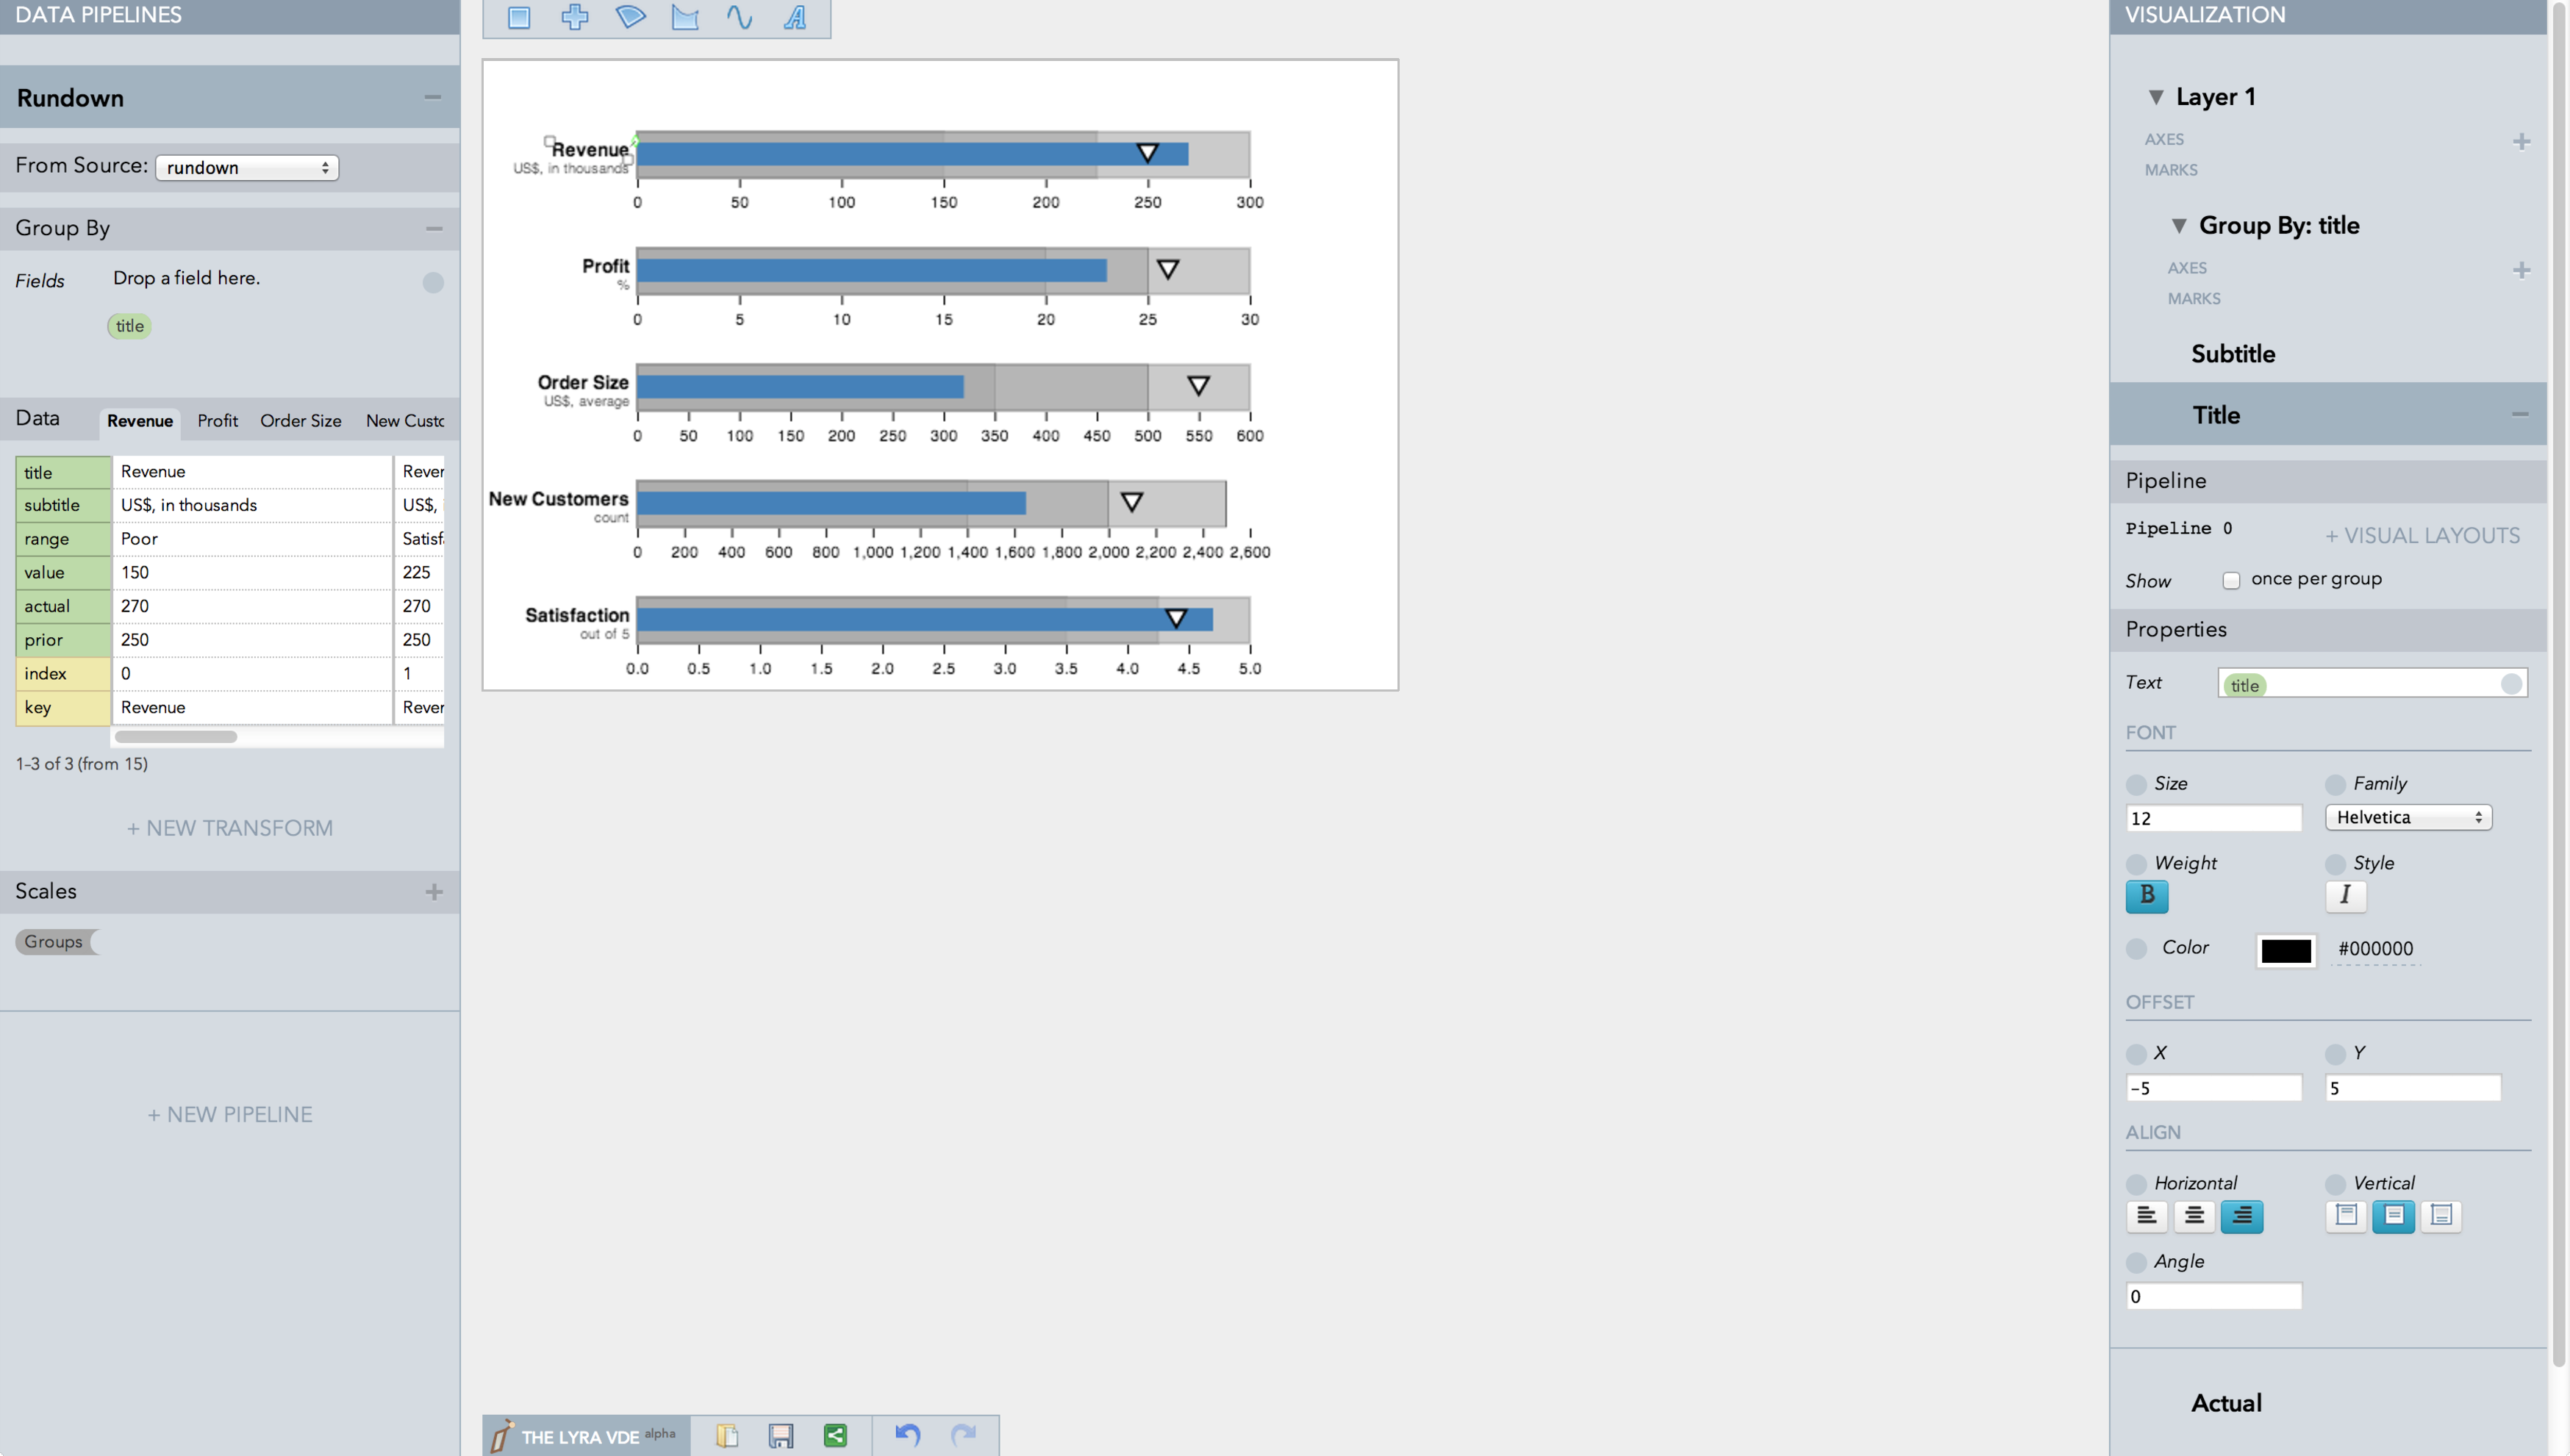
\includegraphics[width=\columnwidth]{bullet_chart}
  \caption{Bullet chart using rectangle and symbol marks grouped
by category. Labels are positioned via a left-edge connector on rectangles.}
  \label{fig:lyra:bulletChart}
\end{figure}

\begin{figure}[h!]
  \centering
  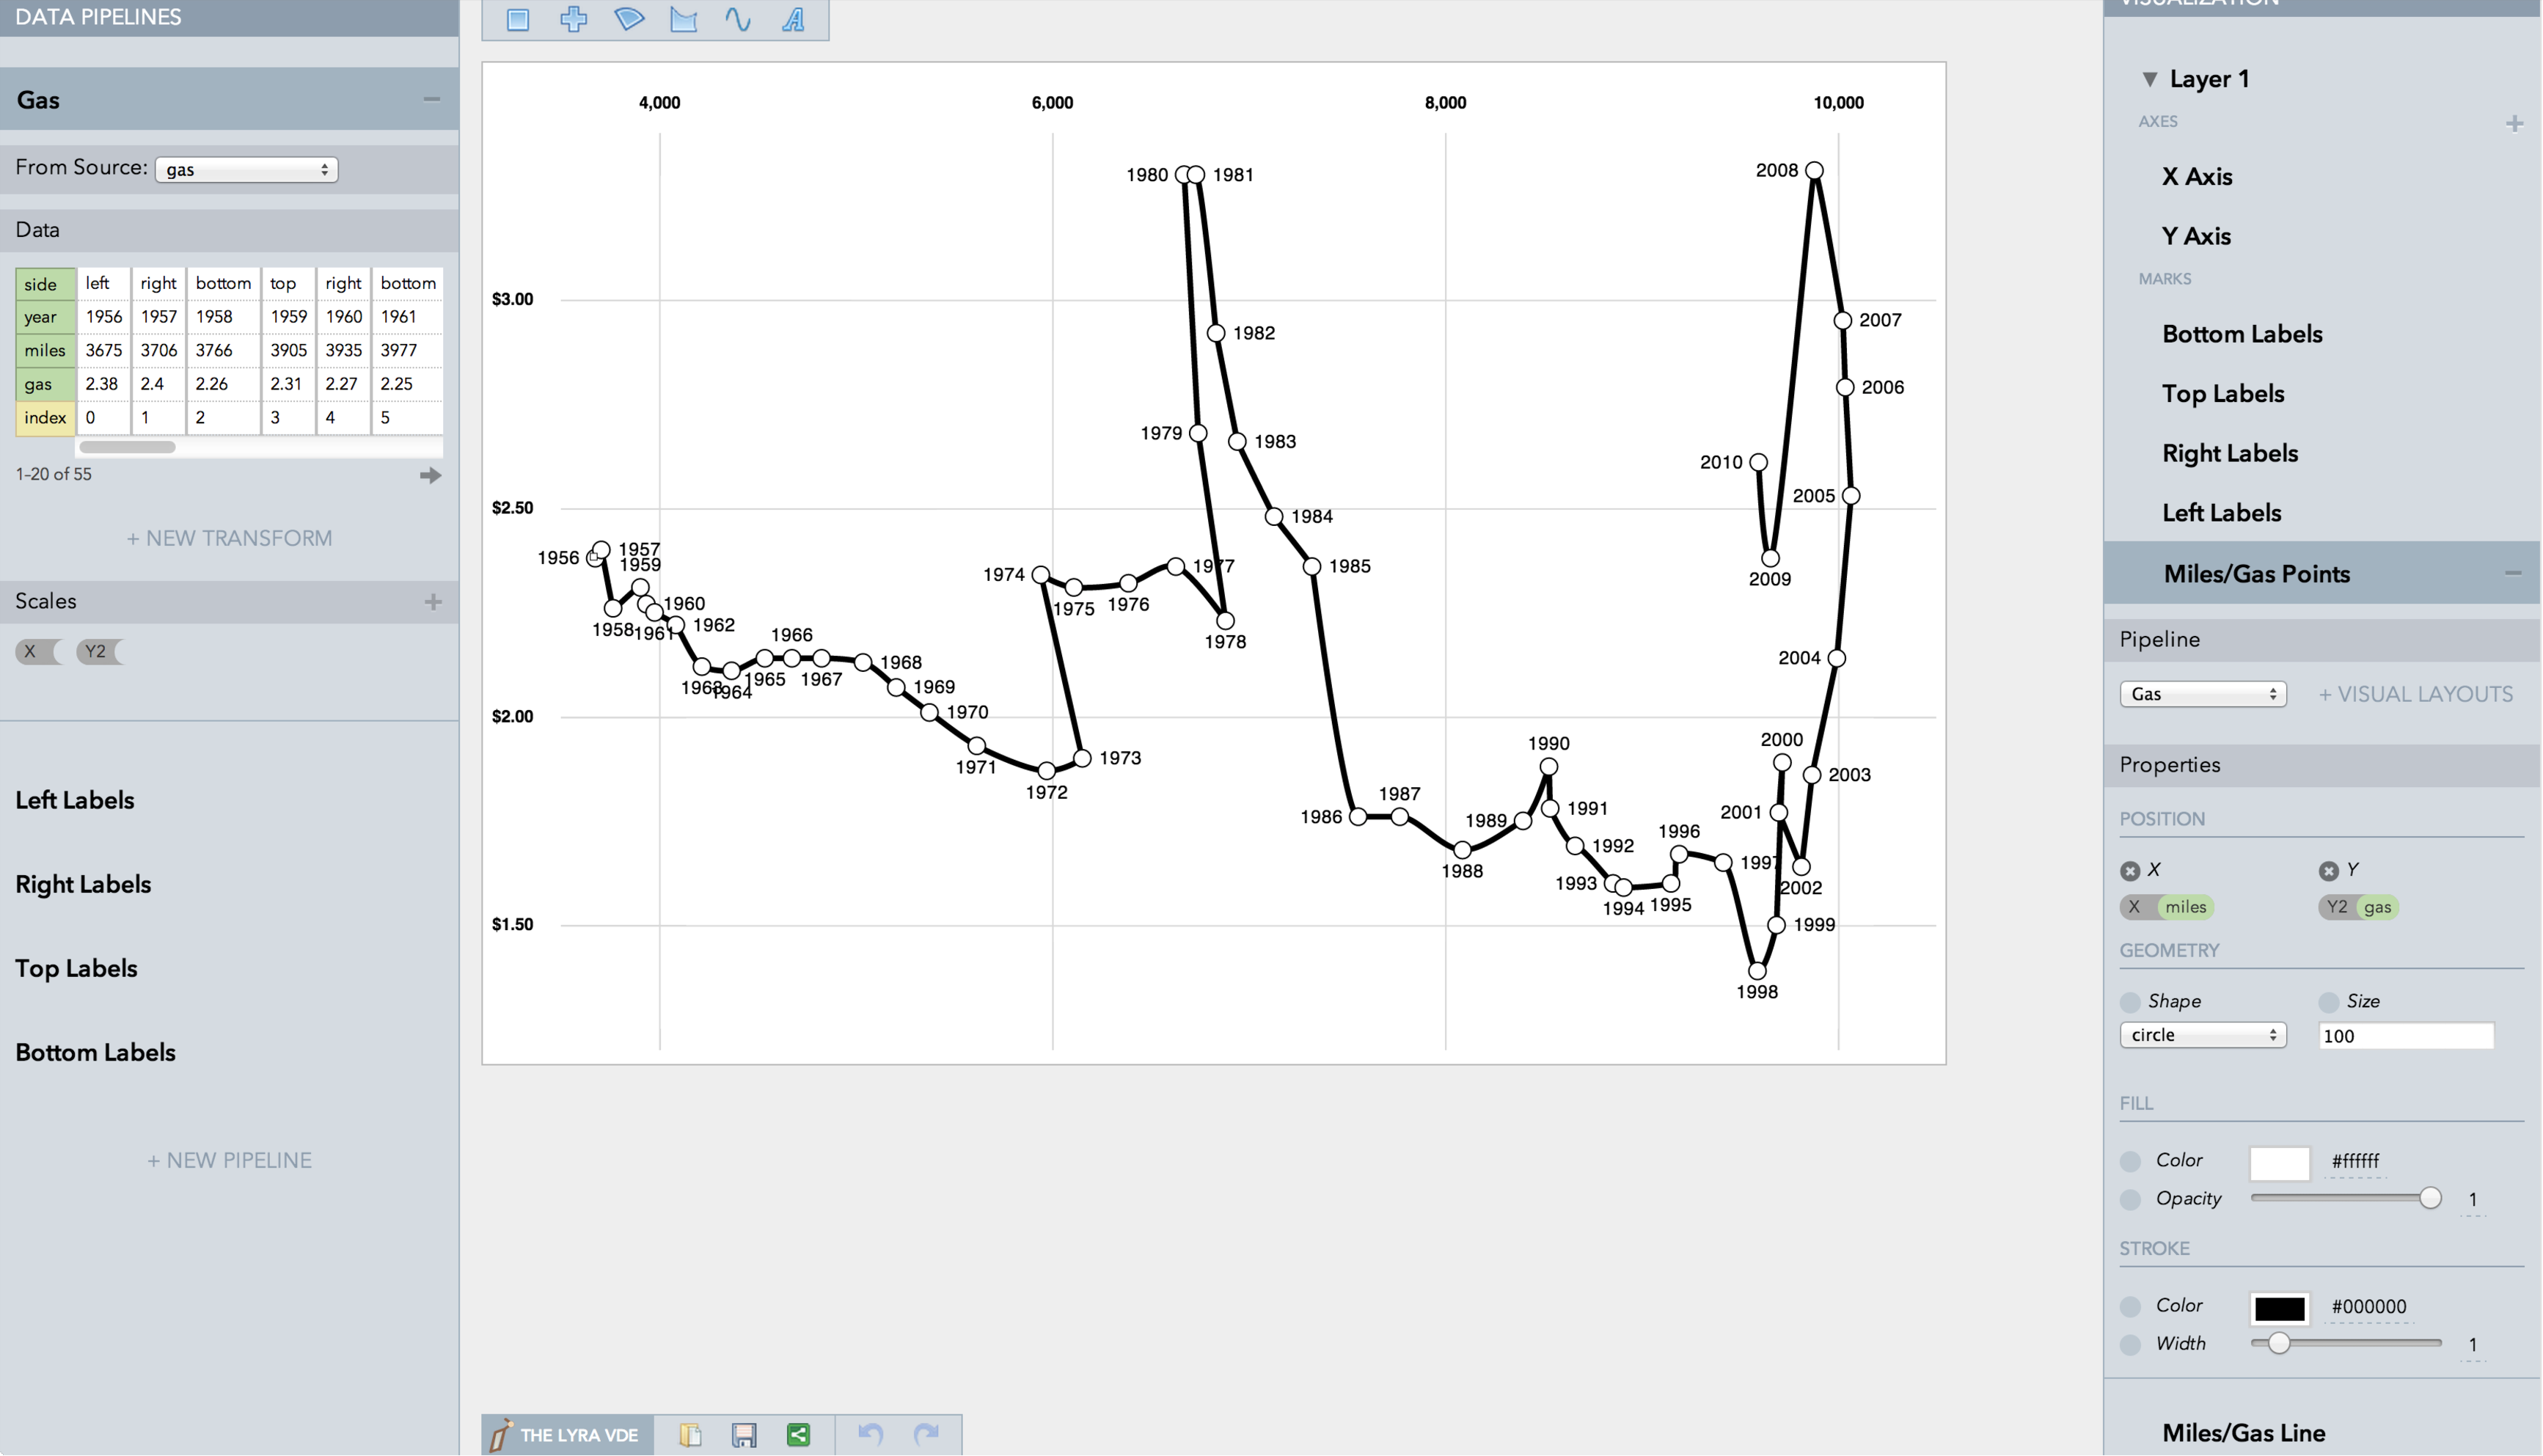
\includegraphics[width=\columnwidth]{driving}
  \caption{A recreation of \emph{Driving Shifts Into Reverse} by Hannah
  Fairfield from The New York Times, originally published May 2, 2010.}
  \label{fig:lyra:gas_driving}
\end{figure}

\begin{figure}[h!]
  \centering
  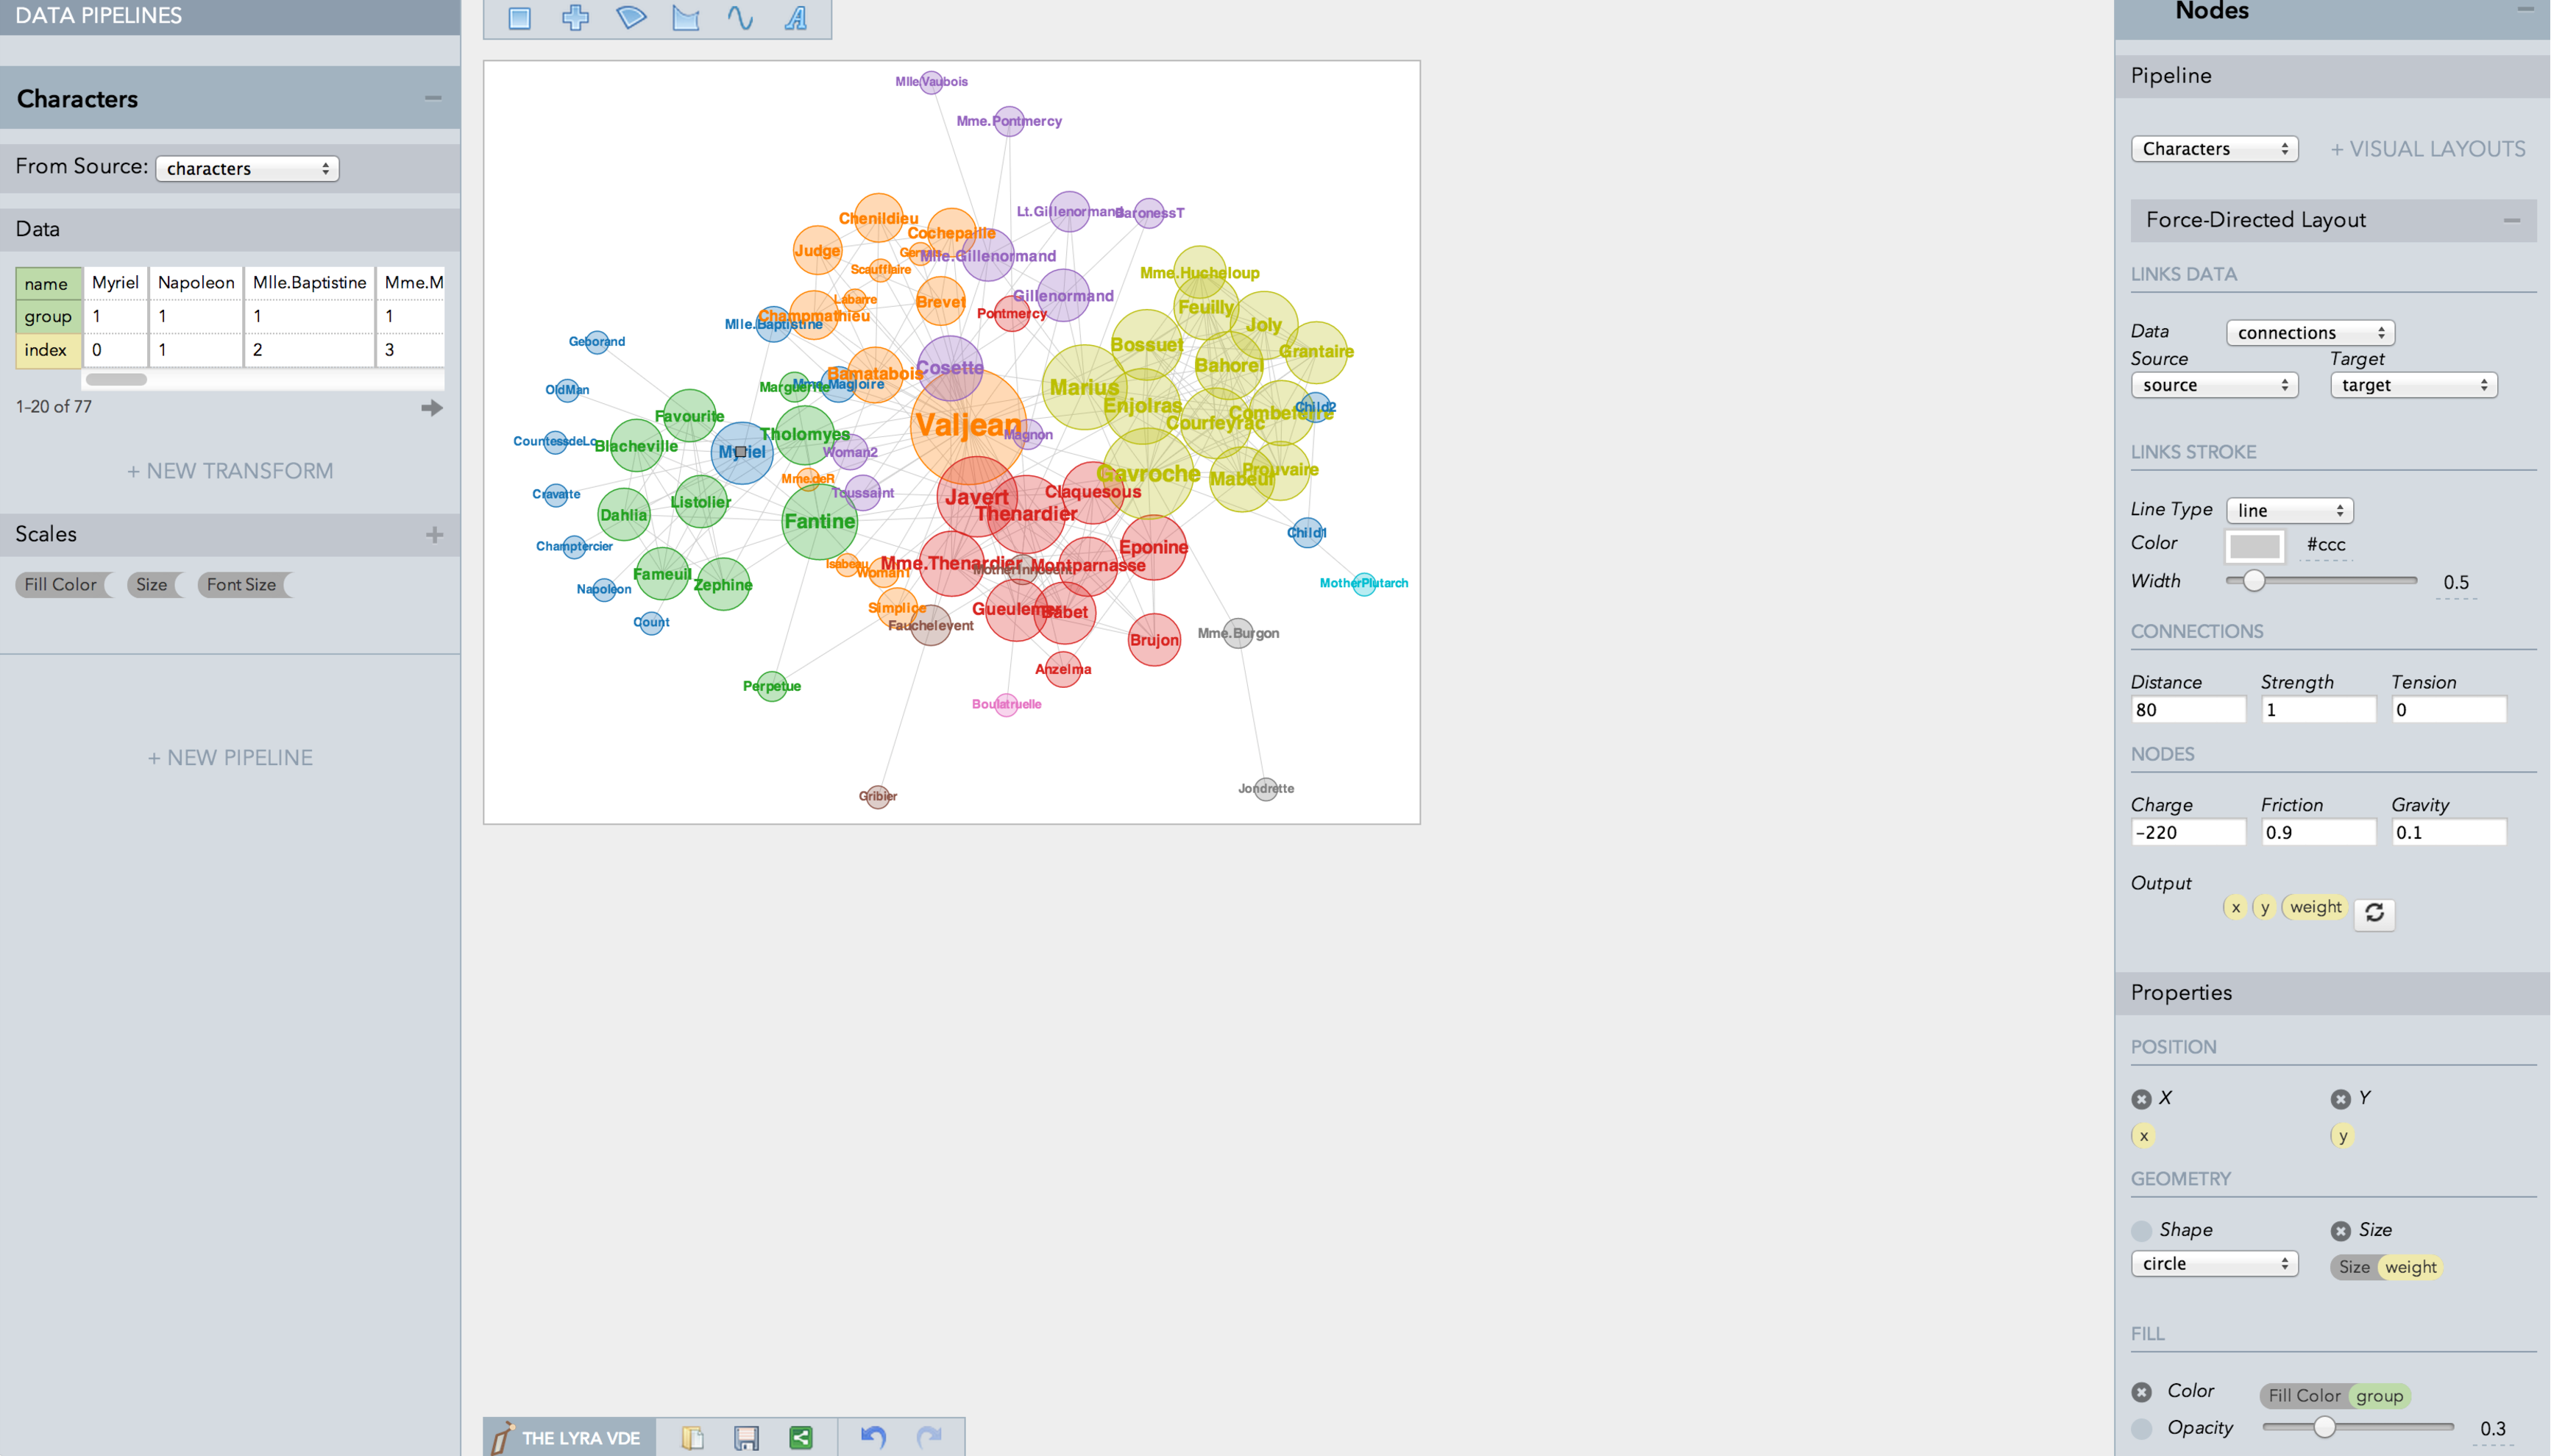
\includegraphics[width=\columnwidth]{les-mis}
  \caption{Character co-occurrences in Les
Mis\'{e}rables. Colors represent cluster memberships computed by a
community-detection algorithm.}
  \label{fig:lyra:les_mis}
\end{figure}

\begin{figure}[h!]
  \centering
  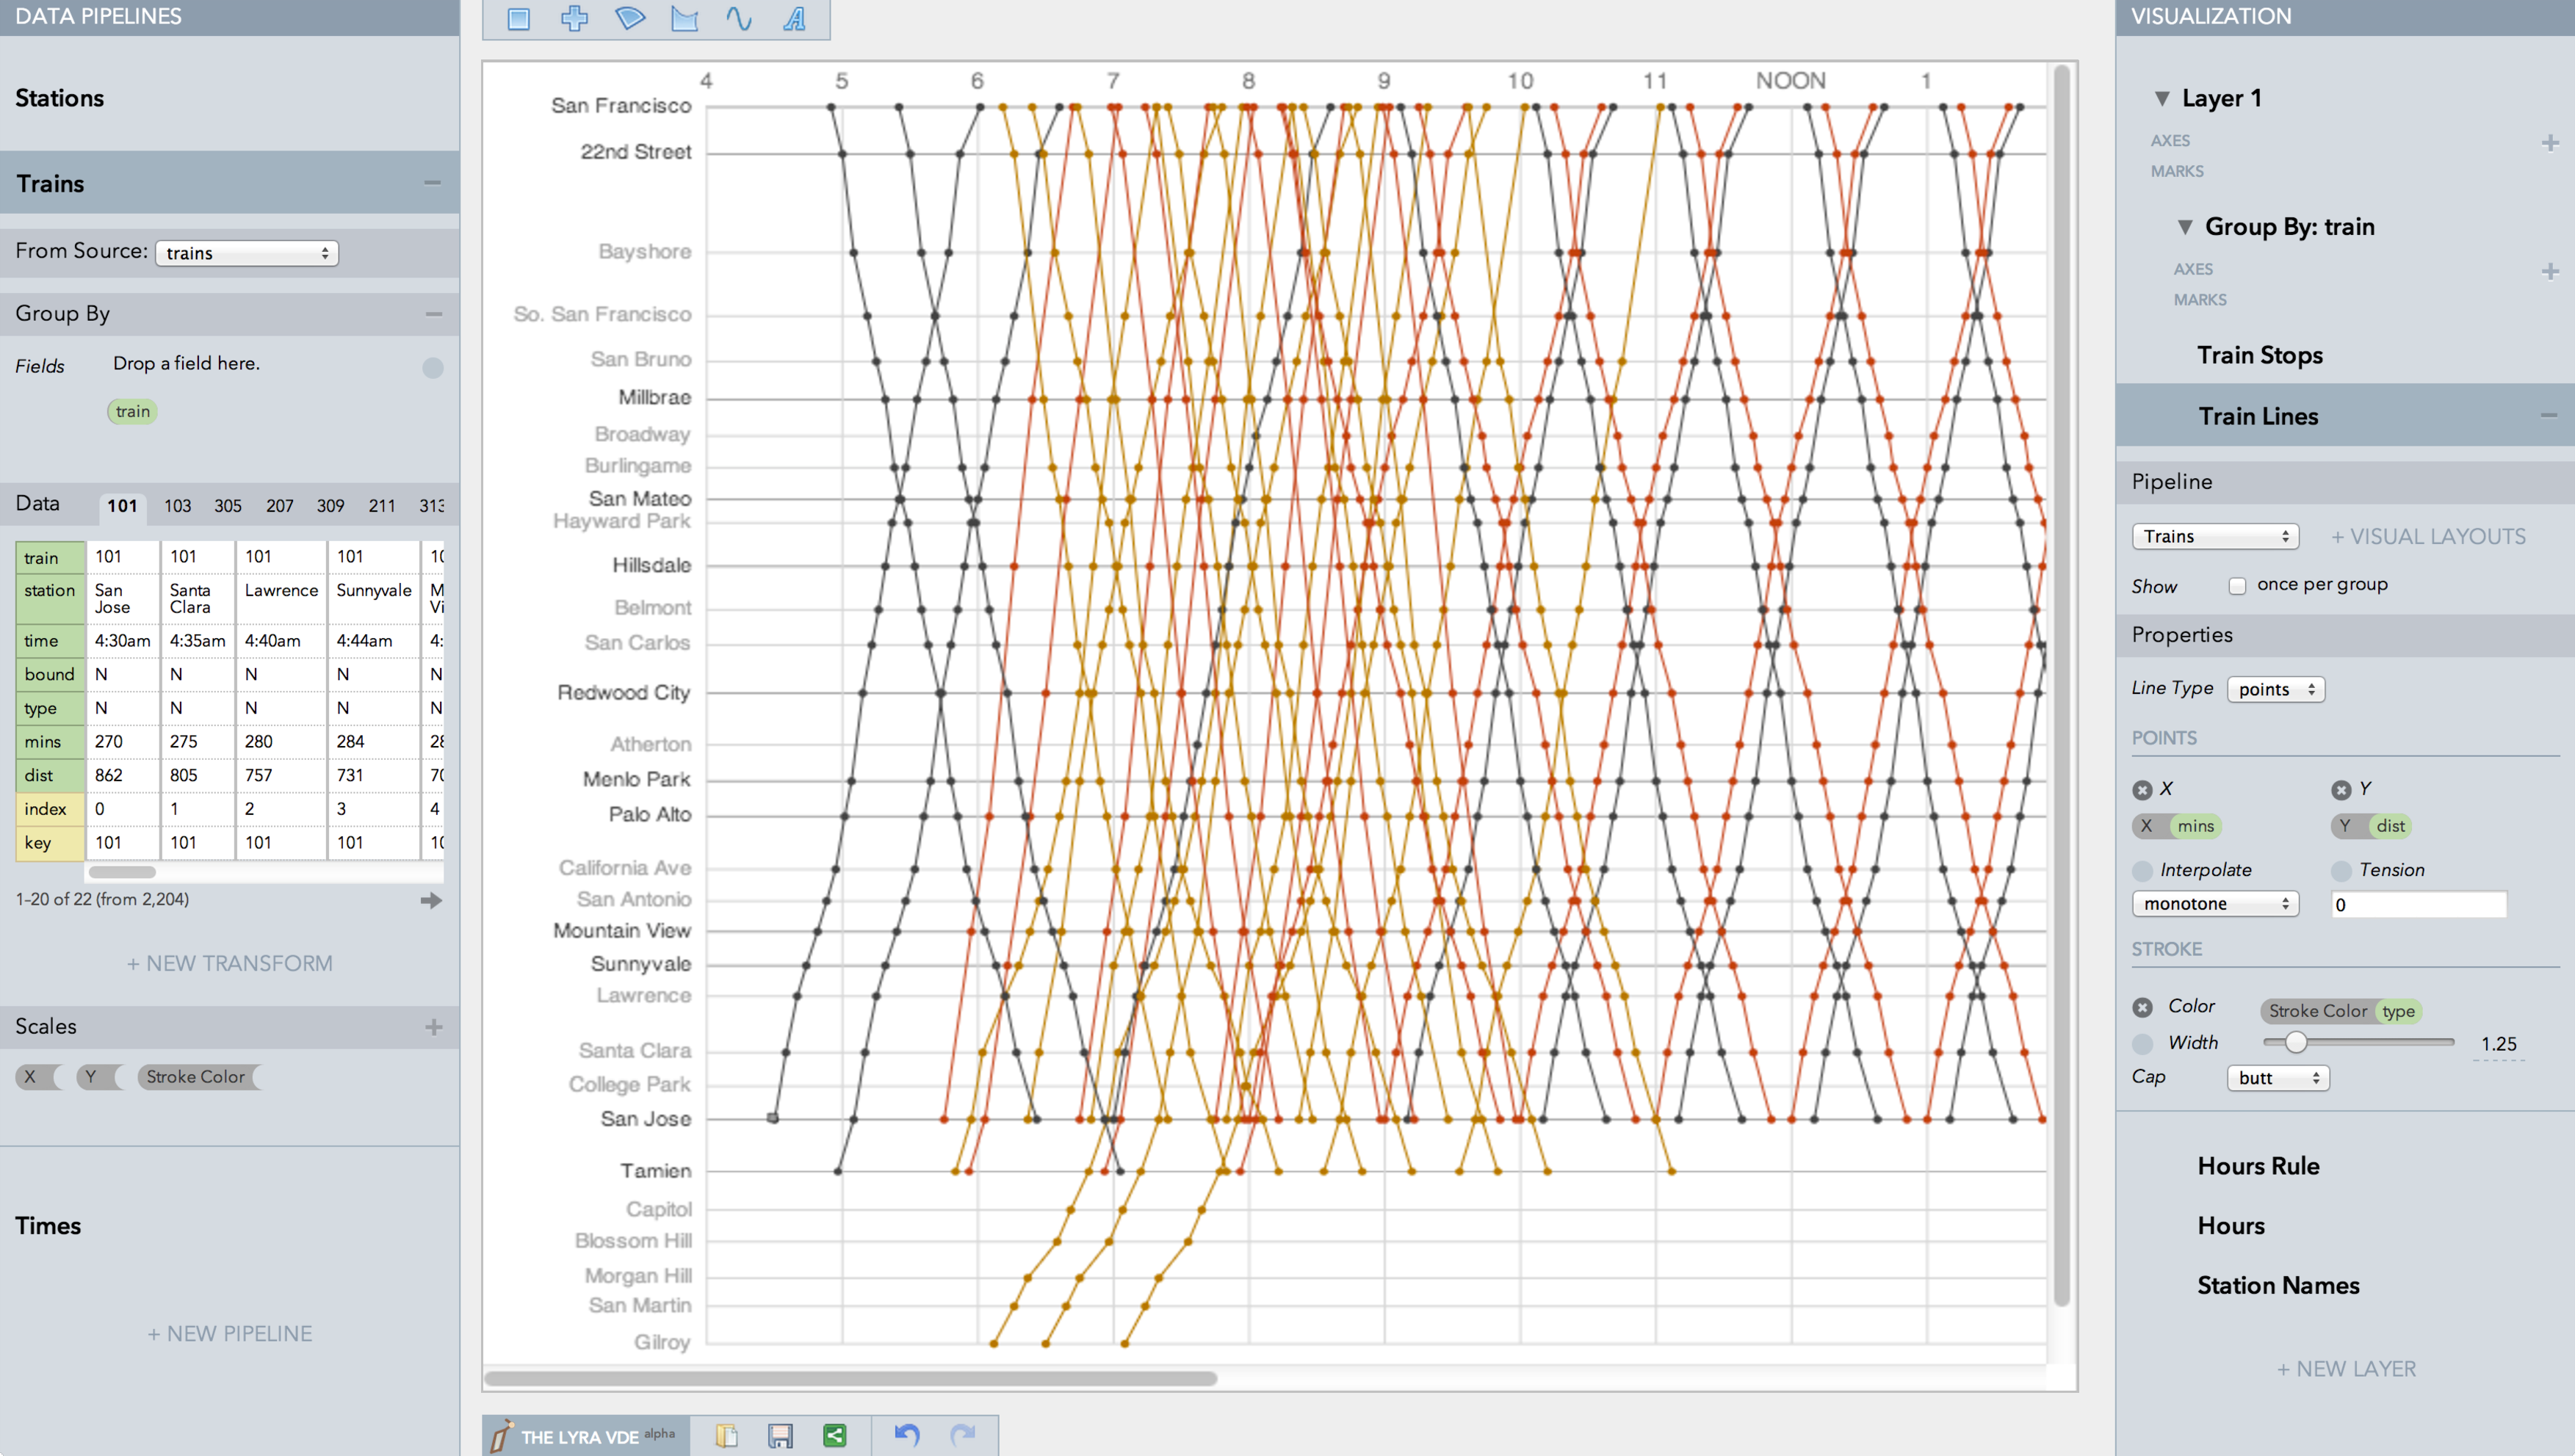
\includegraphics[width=\columnwidth]{caltrain}
  \caption{The schedule of the San Francisco Bay Area's CalTrain service in the style of E. J. Marey's Paris train schedule.}
  \label{fig:lyra:caltrain}
\end{figure}

\begin{figure}[h!]
  \centering
  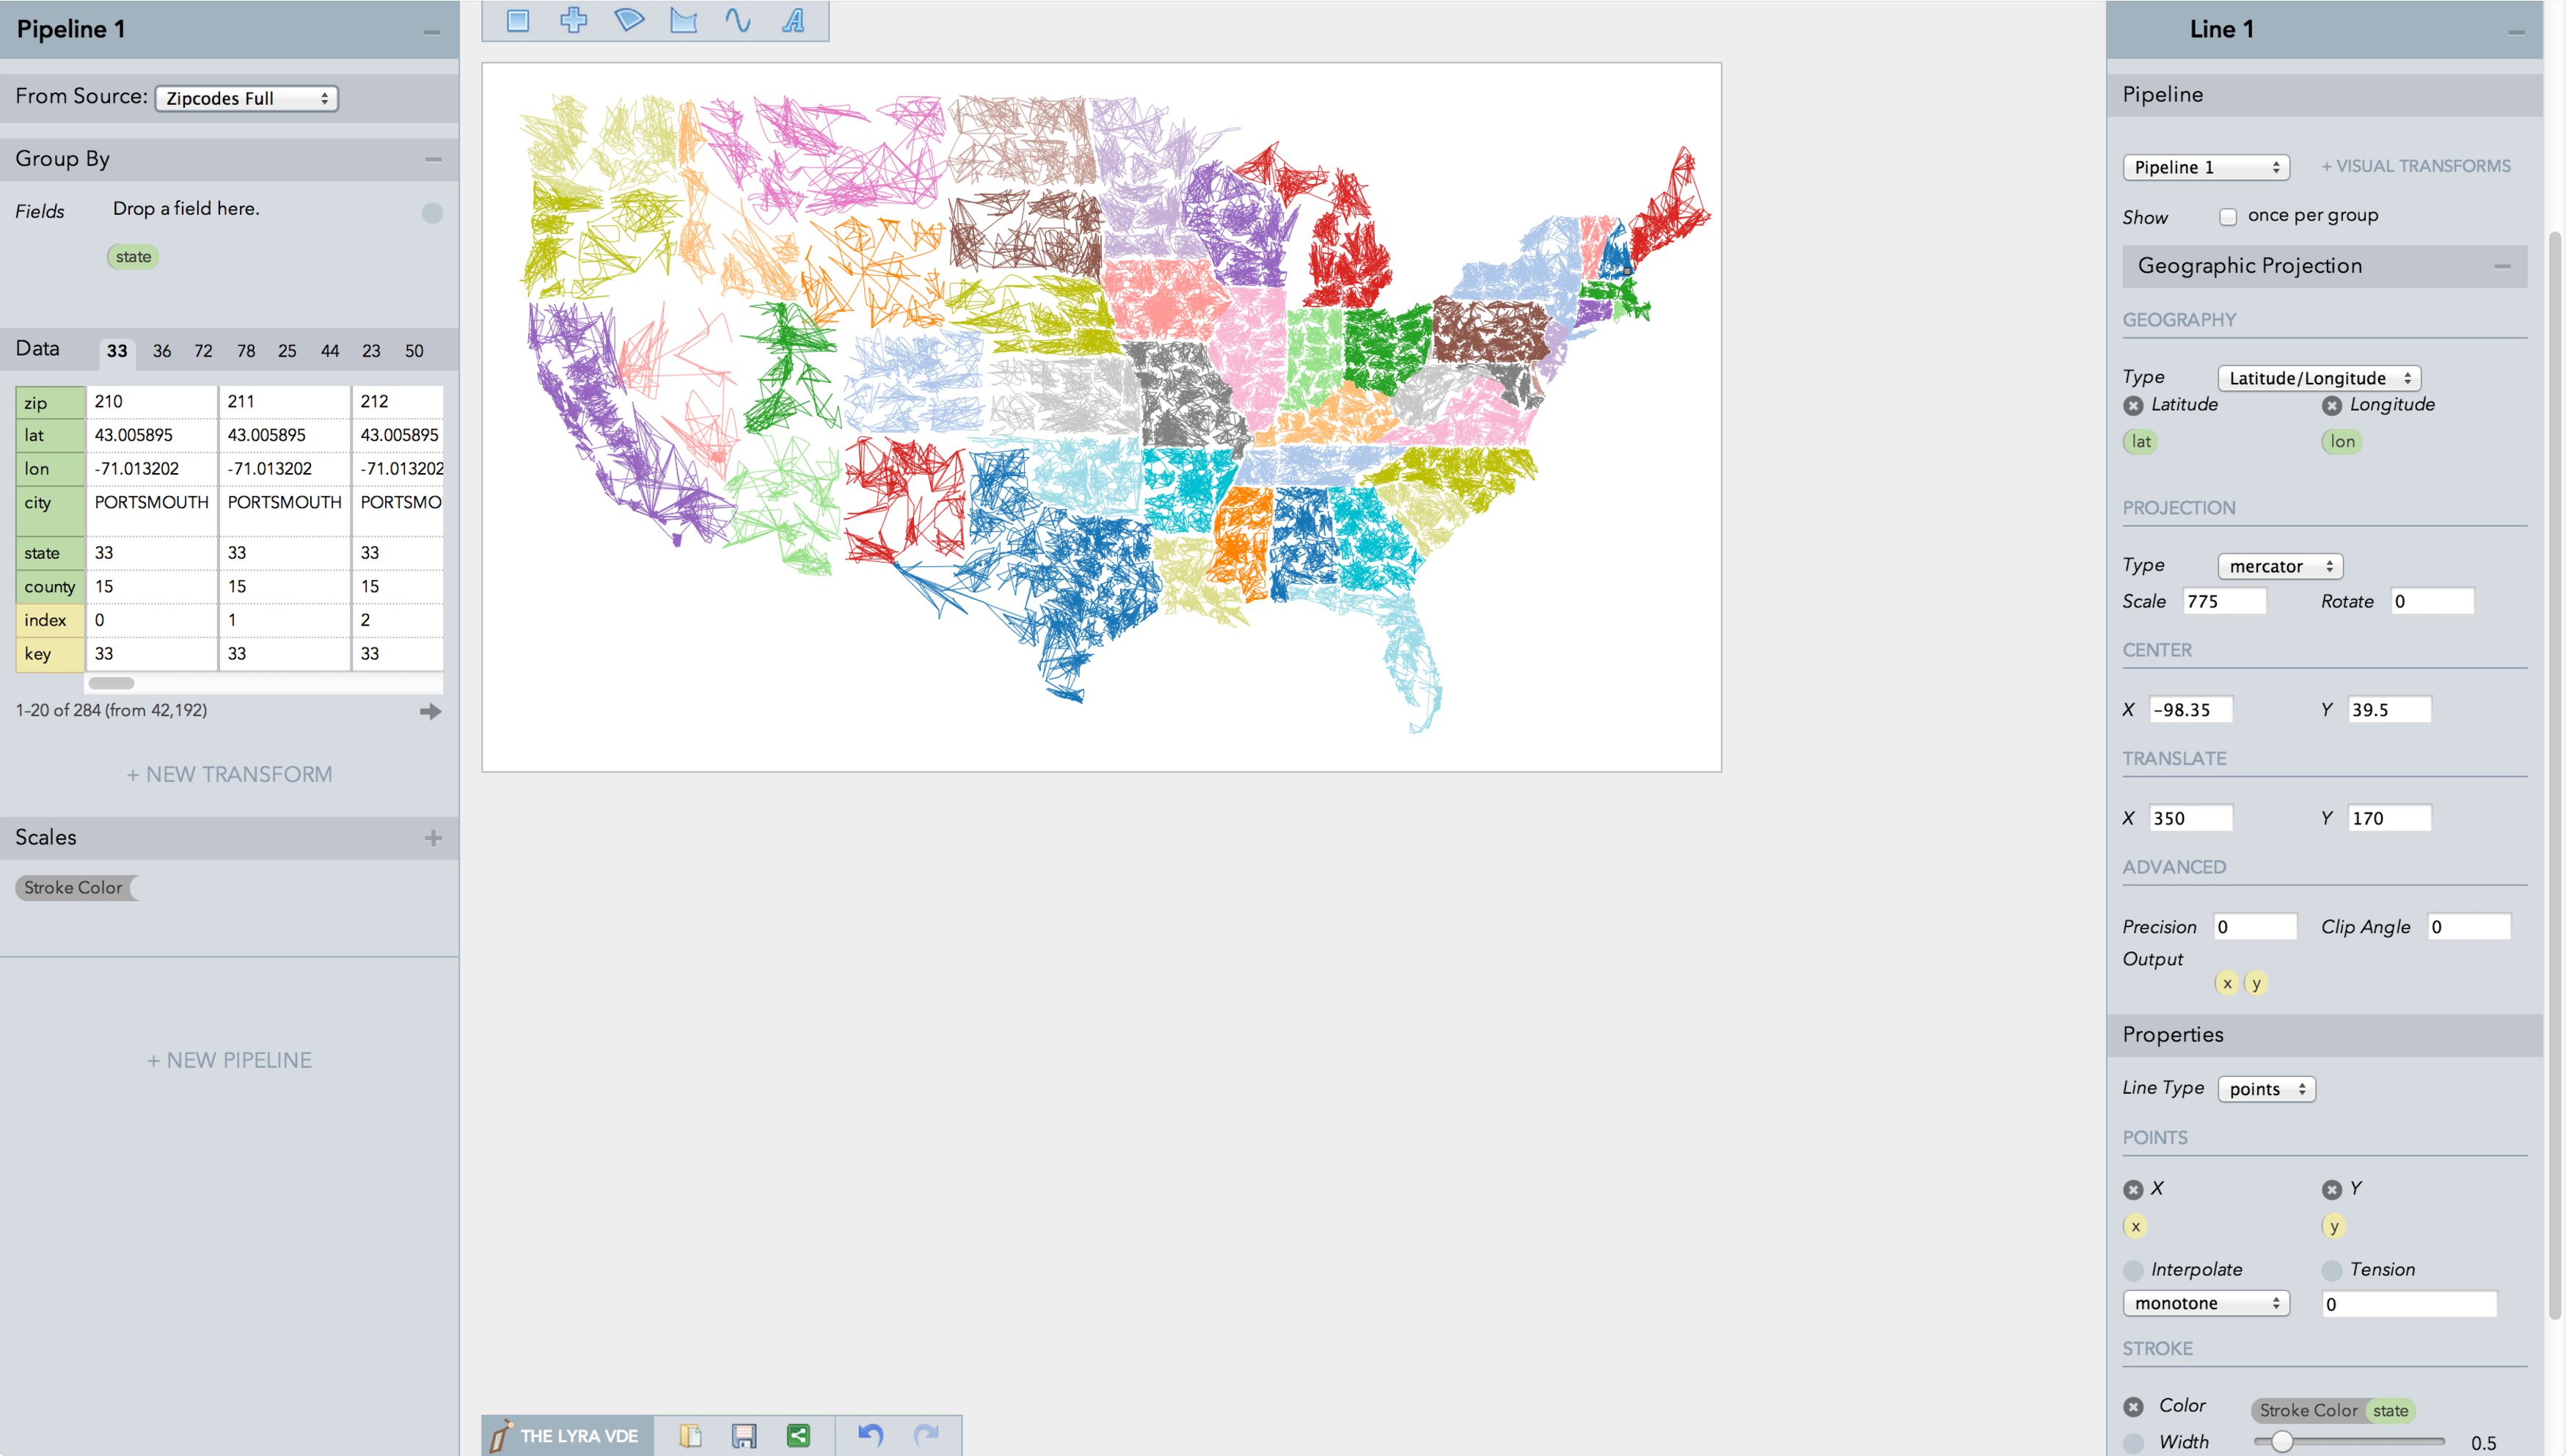
\includegraphics[width=\columnwidth]{zipscribble}
  \caption{ZipScribble by Kosara~\cite{kosara:zipscribble}. A \emph{geo} layout
 encoder is used with line marks to connect latitude and longitudes of zip
 codes.}
  \label{fig:lyra:zipscribble}
\end{figure}

\begin{figure}[h!]
  \centering
  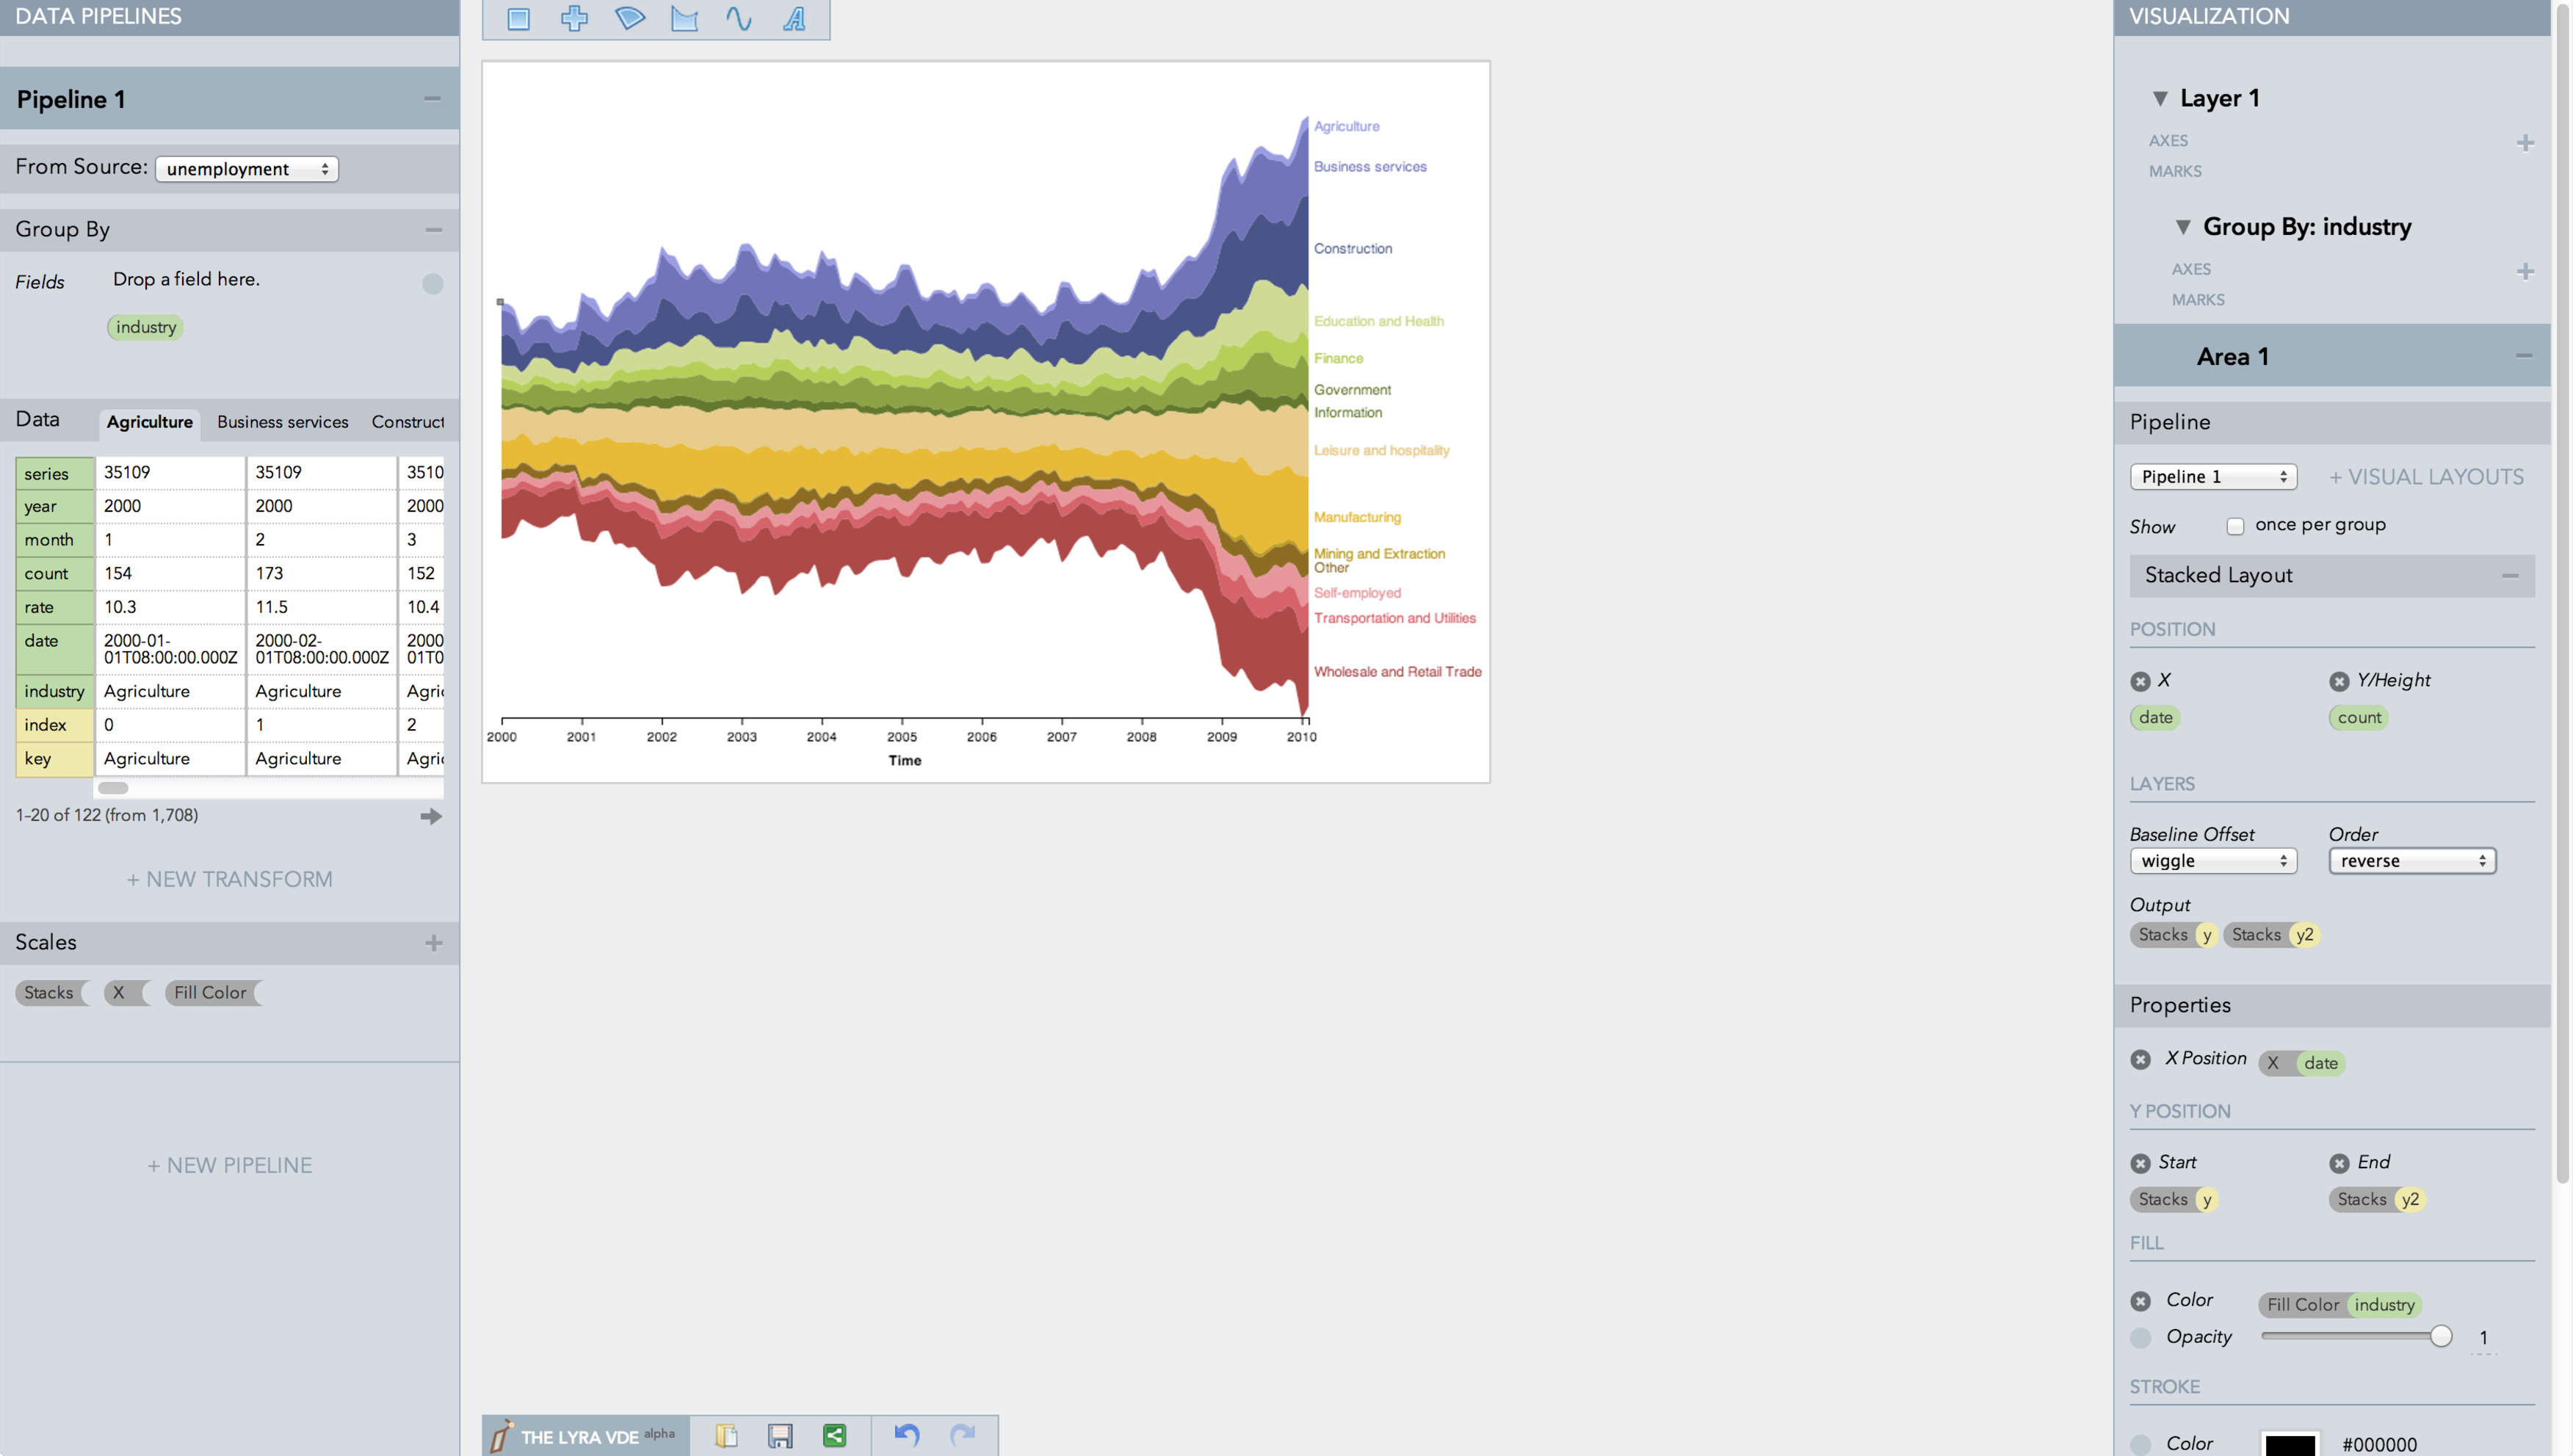
\includegraphics[width=\columnwidth]{streamgraph}
  \caption{A streamgraph of unemployed U.S. workers by industry, using a
  \emph{stack} layout with a \texttt{wiggle} offset~\cite{byron:streamgraph}.}
  \label{fig:lyra:streamgraph}
\end{figure}

\begin{figure}[h!]
  \centering
  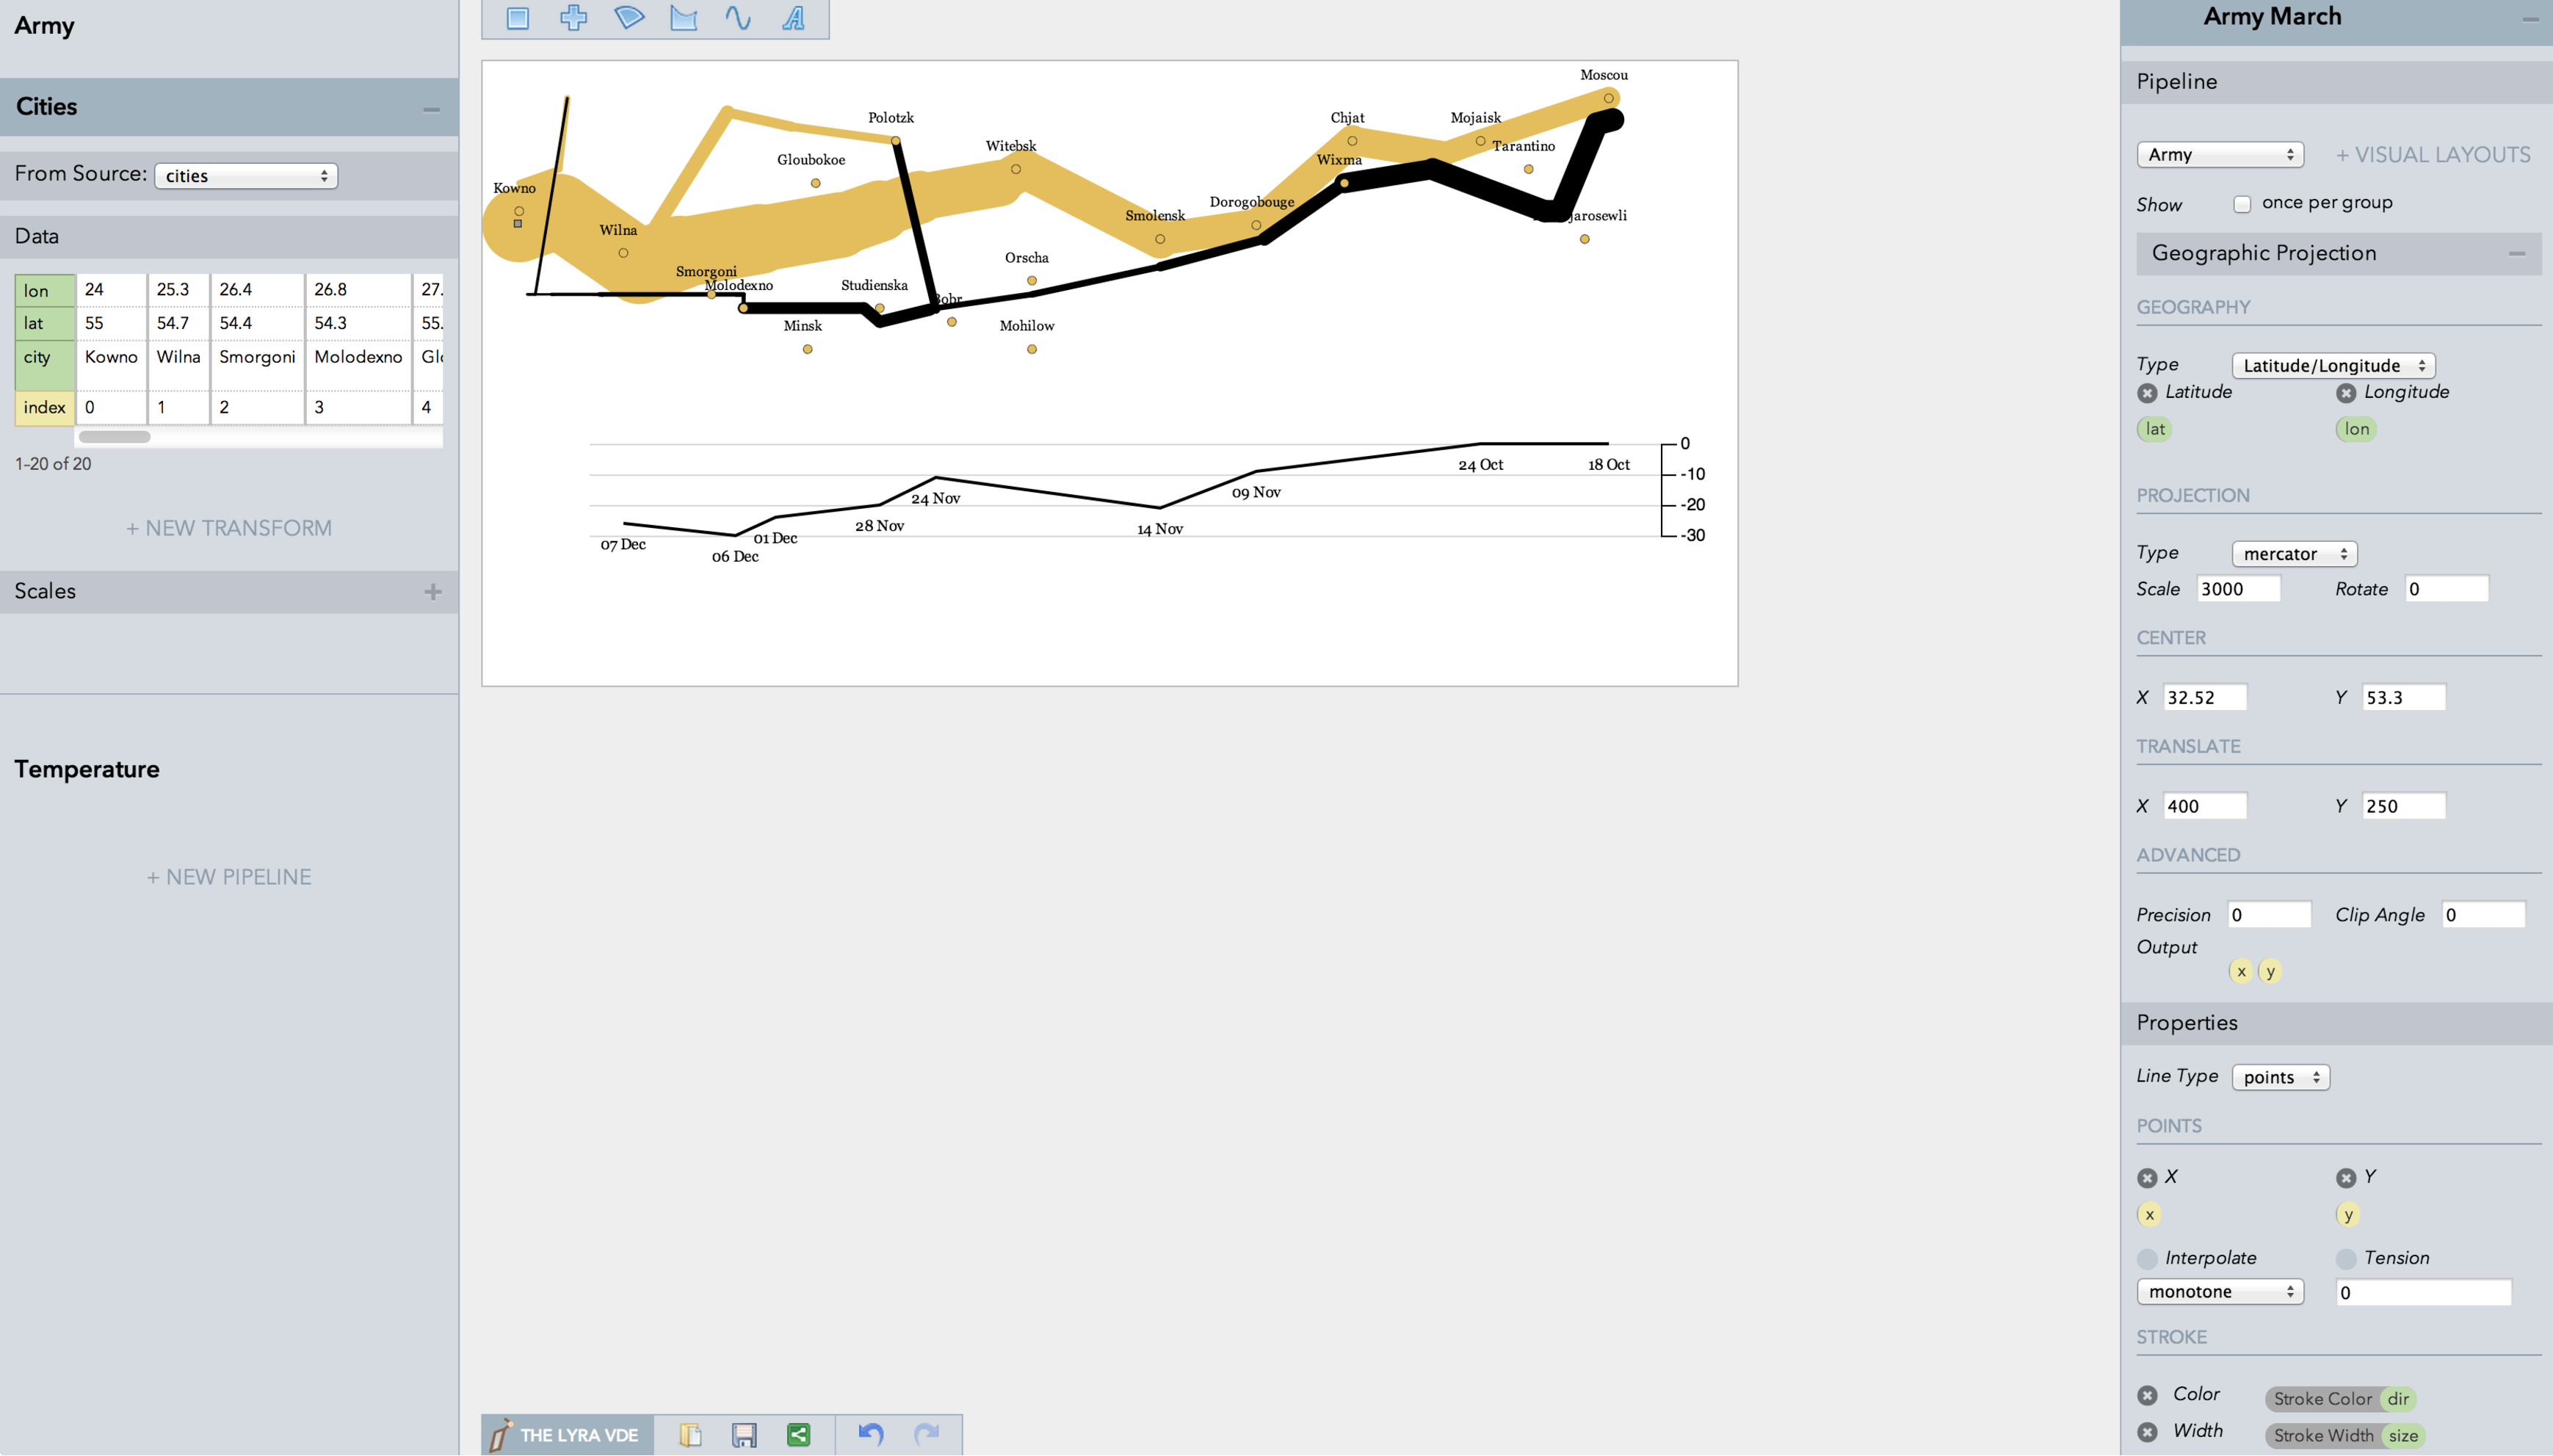
\includegraphics[width=\columnwidth]{napoleon}
  \caption{Minard's map of Napoleon's Russian campaign. A \emph{geo} transform
 encodes spatial positions; army size maps to line stroke width.}
  \label{fig:lyra:napoleon}
\end{figure}

\begin{figure}[h!]
  \centering
  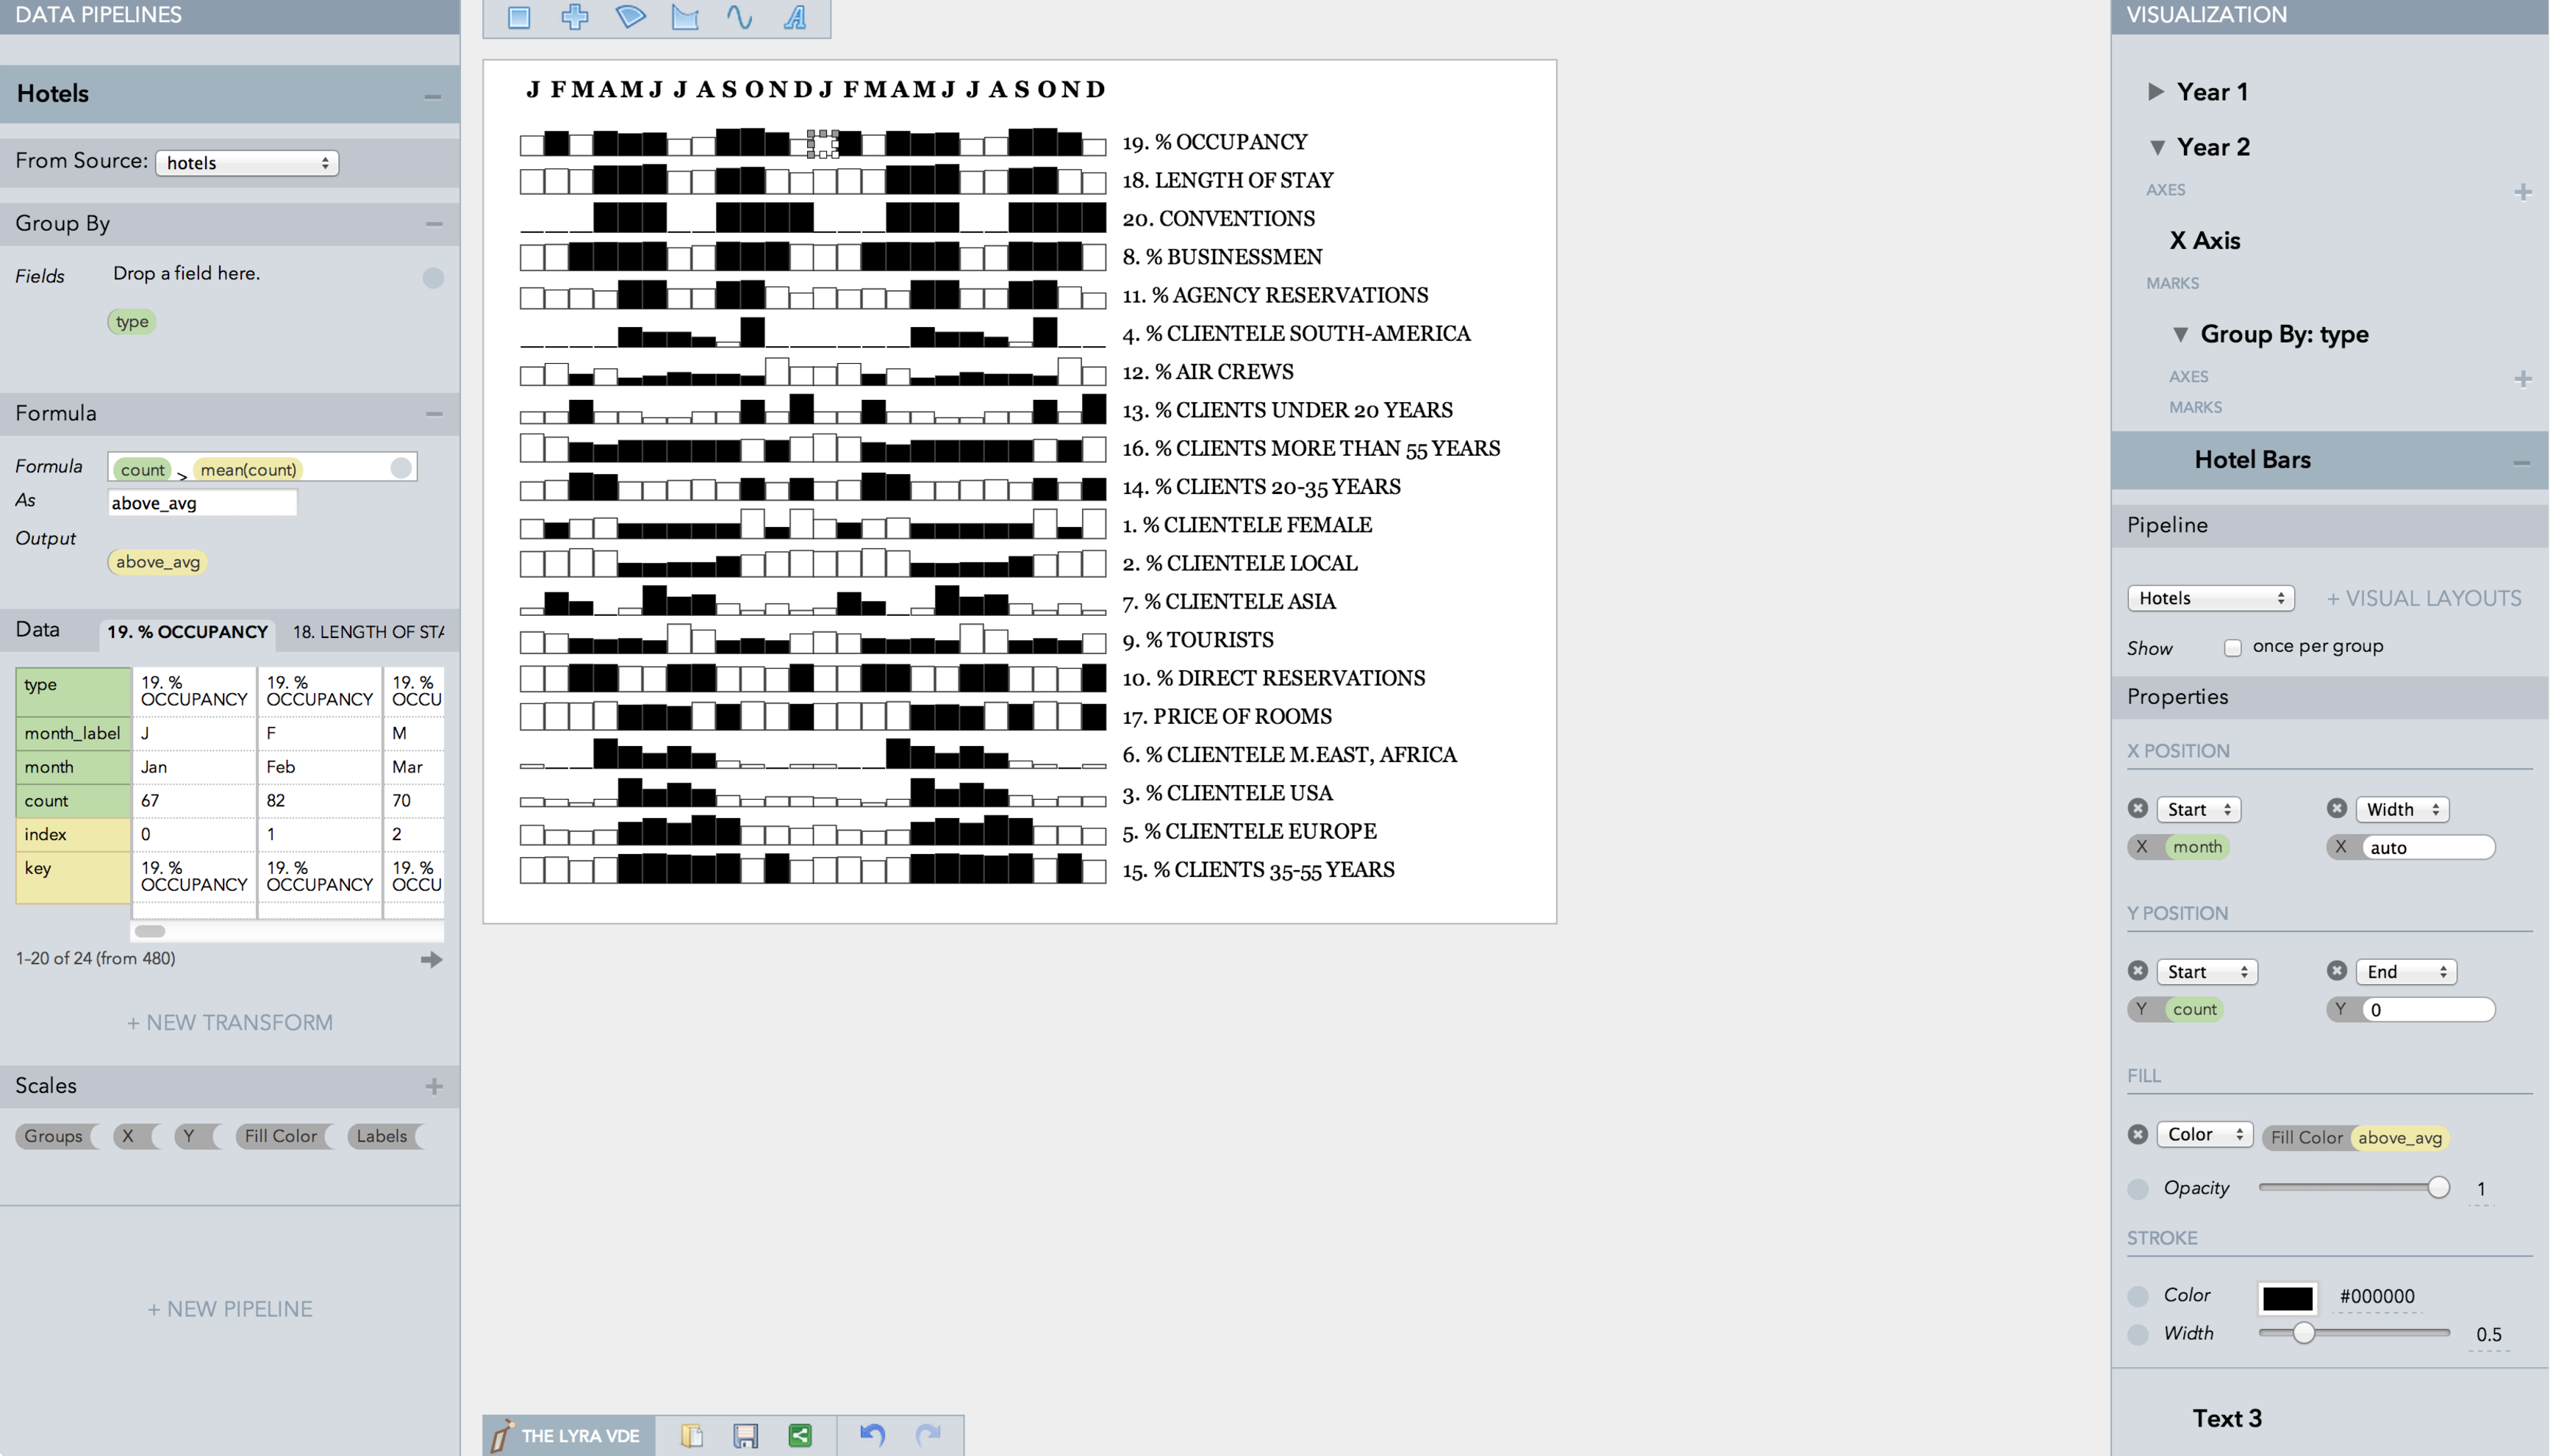
\includegraphics[width=\columnwidth]{bertin}
  \caption{Jacques Bertin's analysis of hotel patterns. \emph{Group by} and \emph{formula}
 transforms are used to shade bars with values above the mean.}
  \label{fig:lyra:bertin}
\end{figure}

\clearpage

\subsection{Limitations}

\vspace{-7pt}

\Cref{fig:lyra:usage,fig:lyra:bulletChart,fig:lyra:gas_driving,fig:lyra:les_mis,fig:lyra:caltrain,fig:lyra:zipscribble,fig:lyra:streamgraph,fig:lyra:napoleon,fig:lyra:bertin}
demonstrate that Lyra enables an expressive design space, but creating these
examples also reveals some limitations. Vega currently lacks support for polar
coordinates. As a result, Lyra cannot (yet) provide \emph{arc} mark connectors
or produce radial axes, making it difficult to recreate classic visualizations
such as Nightingale's Rose or Burtin's antibiotics chart. Additionally, Lyra
only supports the \textsc{rgb} color space, while Vega also supports
\textsc{hsl}, \textsc{lab}, and \textsc{hcl}. These color spaces facilitate
perceptually-sound designs. We plan to address these limitations in future
versions of Vega and Lyra.